\newcommand{\realizable}{\textsc{realizable}}
\newcommand{\unrealizable}{\textsc{unrealizable}}
\newcommand{\skolems}{\textit{Skolems}}
\newcommand{\init}{\textit{Init}}
\newcommand{\isValid}{\textsc{isValid}\xspace}
\newcommand{\isInvalid}{\textsc{isInvalid}\xspace}
%\newcommand{\isSat}{\textsc{isSat}\xspace}
\newcommand{\isUnsat}{\textsc{isUnsat}\xspace}


% \newcommand{\synthesisalgorithm}{
% \begin{algorithm2e}[H]
% \SetAlFnt{\tiny}
% \SetAlCapFnt{\small}
% \SetAlCapNameFnt{\small}
% \SetAlgoSkip{}
% \SetKwFor{While}{forever}{do}{}
% \SetKw{KwContinue}{continue}
% \KwIn{Assume-Guarantee Contract in Lustre, $(A,G)$}
% \KwOut{Skolem collection \skolems, \\ \hspace{+1.3cm} Return value $\in
% \{\realizable, \unrealizable\}$ of ${(A,G)}$.
% }
% \BlankLine
% $i \gets 0$;\\
% $BaseResult \gets \textsc{BaseCheckEngine.\aeval}(BaseCheck(i))$\;
% $ExtendResult \gets \textsc{ExtendCheckEngine.\aeval}(ExtendCheck(i))$;
% \\
% \While{}{	
% 	\uIf(\label{alg:returnUnsat}){(\textsc{BaseCheckEngine}.\isValid($BaseResult$))}
% 	{
% 		\Return
% 		\unrealizable
% 	}
% 	$Skolems.Add(BaseResult.Skolem)$;\\
% 	\uIf(\label{alg:returnSat}){$(\textsc{ExtendCheckEngine}.\isInvalid($ExtendResult$))$}
% 	{
% 		$Skolems.Add((ExtendResult.Skolem))$;\\
% 		\Return \skolems, \realizable
% 	}
% 	$i$++;
% }
% \caption{Synthesis from Assume-Guarantee Contracts}
% \label{alg:synthesis}
% \end{algorithm2e}
% }


\section{Synthesis from Assume-Guarantee Contracts}
\label{sec:synthesis}

%GRIGORY: no need to repeat the things since they all are mentioned in the intro (a couple of paragraphs above)
%
In this section we provide %a summary of the formal background
%that has already been established in previous work, regarding an algorithm that
%is able to generate leaf-level component implementations using only the
%information provided by the user through requirements expressed in the form of an
%Assume-Guarantee contract. Our approach supports the Linear Real
%Arithmetic (LRA) theory.
%mainly due to the limitations imposed by the underlying machinery.
% We begin with
a brief background on Assume-Guarantee contracts,
proceed with summarizing our earlier results on realizability
checking of contracts, and finally
present our program synthesis procedure.
%Finally, we enrich our formal definitions with an informal proof of the
%algorithm's correctness in terms of the successfully synthesized
%implementations.

\subsection{Assume-Guarantee Contracts}

One popular way to describe software requirements is through Assume-Guarantee contracts, where requirements are expressed using safety properties that are split into two categories. The \emph{assumptions} of the contract correspond to properties that restrict the set of valid inputs a system can process, while the \emph{guarantees} dictate how the system should behave through constraints on the outputs that are produced by the system.

For example, consider the contract with the assumption $A = \{x\neq
y\}$ and the guarantee $G = \{x \leq y \Longrightarrow z =
\textit{true}, x \geq y \Longrightarrow z = \textit{false}\}$, for a component with two inputs $x$ and $y$ and one output $z$.  By assumption, $x \neq y$, so the implemented system should set $z$ to true if $x < y$ and false otherwise.  %Although this contract is trivial to implement, the contract does not provide an implementation, only a specification.
%
Determining whether an implementation can be constructed to satisfy the contract for all possible input sequences is the \emph{realizability} problem, while automatically constructing a witness of the proof of
realizability of the contract is the \emph{program synthesis} problem.  The contract $(A,G)$ above is obviously \emph{realizable}, and therefore an implementation can be constructed.
However, if the assumption is omitted then the contract is \emph{unrealizable}, since there is no correct value for $z$ when $x=y$.

\subsection{Formal Preliminaries}
\label{sec:pre}

We describe a system using the disjoint sets $state$ and $inputs$.
Formally, an \emph{implementation} is a \emph{transition system}
described by an initial state predicate $I(s)$ of type $state \to
bool$ and by a transition relation $T(s,i,s')$ of type $state \to
inputs \to state \to bool$.

An Assume-Guarantee (AG) contract can be formally defined by a set of
\emph{assumptions} and a set of \emph{guarantees}. The
\emph{assumptions}, $A: state \rightarrow inputs \rightarrow bool$,
impose constraints over the inputs which may be modal in terms of the
previous state. The \emph{guarantees} $G$ consist of two separate
subsets $G_I: state \rightarrow bool$ and $G_T: state \rightarrow
inputs \rightarrow state \rightarrow bool$, where $G_I$ defines the
set of valid initial states, and $G_T$ specifies the properties that
need to be met during each new transition between two states. Note
that we do not necessarily expect that a contract would be defined
over all variables in the transition system, but we do not make any
distinction between internal state variables and outputs in the
formalism. This way, we can use state variables to (in some cases)
simplify specification of guarantees.

\subsection{Realizability of Contracts}
The synthesis algorithm proposed in this paper is built on top of our realizability algorithm
originally presented in~\cite{Katis15:Realizability}. Using the formal foundations described in Sect.~\ref{sec:pre},
the problem of realizability is expressed using the notion of a state being \emph{extendable}:

\begin{definition}[One-step extension]
\label{def:extend}
A state $s$ is extendable after $n$ steps, denoted $\mathit{Extend}_{n}(s)$, if
any valid path of length $n-1$ starting from $s$ can be extended in response to
any valid input.%
%
\begin{multline*}%
\mathit{Extend}_{n}(s) \triangleq \forall i_1, s_1, \ldots, i_n, s_n.\\ A(s, i_1) \land G_T(s, i_1, s_1)
\land \cdots \land
A(s_{n-1}, i_n) \land G_T(s_{n-1}, i_n, s_n)
\implies \\
\forall i.~ A(s_n, i) \implies \exists s'.~ G_T(s_n, i, s')
\end{multline*}
\end{definition}

The algorithm for realizability uses Def.~\ref{def:extend} in two
separate checks that correspond to the two traditional cases exercised
in k-induction. Initially, we prove that the set of initial states is
not empty, which is done by checking for the existence of at least one
state that satisfies $G_I$. For the $\mathit{BaseCheck}$, we ensure
that all initial states are extendable for any path of length $k < n$,
while the inductive step of $\mathit{ExtendCheck}$ tries to prove that
all valid states are extendable for any path of length $n$. Therefore,
we attempt to find the smallest $n$, for which the two following
$\forall\exists$-formulas are valid:%
%
\begin{equation}
\label{eq:sbcheck}
\mathit{BaseCheck}(n) \triangleq \forall k < n. (\forall s. G_I(s)
	  	\implies \mathit{Extend}_k(s))
\end{equation}%
%
\begin{equation}
\label{eq:echeck}
\mathit{ExtendCheck}(n) \triangleq \forall s. \mathit{Extend}_n(s)
\end{equation}

The realizability checking algorithm has been used to effectively find cases
where the traditional consistency check (i.e. the existence of an assignment
to the input variables for which the output variables satisfy the contract)
failed to detect conflicts between stated requirements in case studies of
different complexity and importance. It has also been formally verified using the Coq proof assistant in terms of its
soundness, for the cases where it reports that a contract is
realizable~\cite{katis2015machine}.

\subsection{Program Synthesis from Proofs of Realizability}

%While the implemented algorithm on realizability provided us with meaningful
%results during the verification of several contracts,
An important outcome of our previous work on realizability is that it
can be further used for solving the more complex problem of
\emph{program synthesis}. That is, we can automatically
derive implementations from the proof of a contract's realizability.
%The limited power of SMT solvers
%in terms of solving formulas containing nested quantifiers immediately ruled
%out the prospect of using one as our primary synthesis tool. Fortunately,
%we are able to exploit our prior results in the scope of solving validity and
%Skolemizing $\forall\exists$-formulas (to be described in Sect.~\ref{sec:aeval}).
%The idea is simple.  
Consider checks~\eqref{eq:sbcheck}
and~\eqref{eq:echeck} that are used in the realizability checking
algorithm. Both checks require that the reachable states explored are
extendable using Def.~\ref{def:extend}. The key insights are then 1)
we can start with a arbitrary state in $G_I$ since it is non-empty, 2)
we can use witnesses from the proofs of $\mathit{Extend}_k(s)$ in
$\mathit{BaseCheck}$ to create a valid path of length $n-1$, and 3) we
can extend that path to arbitrary length by repeatedly using the
witness of the proof of $\mathit{Extend}_n(s)$ in
$\mathit{ExtendCheck}(n)$.

In first order logic, witnesses for valid $\forall\exists$-formulas
are represented by Skolem functions. Intuitively, a Skolem function
expresses a connection between all universally quantified variables in
the left-hand side of the $\forall\exists$-formulas~\eqref{eq:sbcheck}
and~\eqref{eq:echeck} and the existentially quantified variable $s'$
within $\mathit{Extend}$ on the right-hand side. Our algorithm uses
the \aeval tool, detailed in Sect.~\ref{sec:aeval}, to generate such
Skolem functions from the validity of~\eqref{eq:sbcheck}
and~\eqref{eq:echeck}.

%\synthesisalgorithm

%% During the k-induction algorithm, two parallel
%% engines (\textsc{BaseEngine, ExtendEngine}) handle the base and
%% inductive step checks of validity of $\forall\exists$-formulas.
%% The proof of a formula's validity is closely tied to the process of
%% Skolemization: for every step that \textit{BaseCheck(n)} is valid,
%% \aeval provides a Skolem function to witness that validity.

\begin{figure}[t]
\begin{minipage}{0.65\textwidth}
\scalebox{0.8}{
\begin{algorithm2e}[H]
\SetAlgoSkip{}
\SetKwFor{For}{for}{do}{}
\KwOut{$Result: \{\realizable, \unrealizable\}$, \init: state,
\skolems: Skolem list
}
\BlankLine
$Skolems \gets \langle \rangle$; \\ 
$InitResult \gets $\sc{Sat?}$(G_I)$; \\
\uIf(\label{alg:initState}){$(\isUnsat(InitResult))$}
	{%
		\Return
		\unrealizable, $\emptyset$, $\langle \rangle$;%
	}
$\init \gets InitResult.model$; \\
\For{$(i \gets 0; \mathbf{true}; i \gets i + 1)$}{	
$ExtendResult \gets \textsc{\aeval}(ExtendCheck(i))$;
\\
\uIf(\label{alg:returnSat}){$(\isValid(ExtendResult))$}
{
	$Skolems.Add(ExtendResult.Skolem)$;\\
	\Return \realizable, \init, \skolems;
}
$BaseResult \gets \textsc{\aeval}(BaseCheck_{k}(i))$\;
\uIf(\label{alg:returnUnsat}){$(\isInvalid(BaseResult))$}
	{%
		\Return
		\unrealizable, $\emptyset$, $\langle \rangle$;%
	}
$Skolems.Add(BaseResult.Skolem)$;\\

}
\caption{Synthesis from AG-Contracts}
\label{alg:synthesis}
\end{algorithm2e}}
\end{minipage}
\hspace{-0.8cm}
\begin{minipage}[t]{0.38\textwidth}
\scalebox{.8}{
\begin{template}[H]
\SetAlgoSkip{}
\SetKwFor{While}{forever}{do}{}
\BlankLine
  \textsc{assign\_Init()};

\BlankLine
  \textsc{read\_inputs()}\; 		
  \textsc{Skolems}[0]()\;
  $\ldots$\\
  \textsc{read\_inputs()}\;
  \textsc{Skolems}[k-1]()\;

\BlankLine

\While{}{
 \textsc{read\_inputs()}\;
 \textsc{Skolems}[k]()\;
 \textsc{update\_history()};
}
\caption{Structure of an implementation}
\label{alg:synt}
\end{template}}
\end{minipage}
%\caption{Synthesis algorithm and structure of implementations}
%\label{fig:synthalg}
\end{figure}

Alg.~\ref{alg:synthesis} provides a summary of the synthesis
procedure. The algorithm first determines whether the set of initial states $G_I$ is non-empty.
Second, it repeatedly attempts to inductively show the realizability of the system, using
\aeval\ to find Skolem witnesses.  The algorithm
repeatedly proves $\mathit{BaseCheck_k(i)}
\triangleq \forall s. G_I(s) \implies \mathit{Extend}_i(s)$ and
accumulates the resulting Skolem functions. If
$\mathit{BaseCheck_k(i)}$ ever fails, we know $\mathit{BaseCheck(i)}$
would also fail and so the system is unrealizable. At the same time,
the algorithm tries to prove $\mathit{ExtendCheck(i)}$. As soon as the
inductive step of $\mathit{ExtendCheck(i)}$ passes, we have a complete
k-inductive proof stating that the contract is realizable. We then
complete our synthesis procedure by generating a Skolem function that
corresponds to the inductive step, and return the list of the Skolem
functions.  Note that in algorithm 1 for a particular depth $k$,
we perform the extends check prior to the base check.
The intuition is that $\mathit{BaseCheck(i)}$ checks
$\forall k < i$; thus, it is one step ``smaller'' than the extends
check and this avoids a special case at $k=0$.

Given a list of Skolem functions, it remains to plug them into
an implementation skeleton as shown in Template~\ref{alg:synt}.
Combination of Lustre models and k-inductive proofs
allow the properties in the model to manipulate the
 values of variables up to $k-1$ steps in the past. Thus,
the first step of an implementation  (method \textsc{assign\_Init()})
 creates an array for each state variable of size $k+1$, where
$k$ is the depth of the solution to Alg.~\ref{alg:synthesis}.
This array represents the depth of history necessary to compute 
the recurrent Skolem function produced by the $\mathit{ExtendCheck}$ process.
The $\mathit{BaseCheck}$ Skolem functions initialize this history.

In each array, the $i$-th element, with $0\leq i \leq k-1$,
corresponds to the value assigned to the variable after the call to
$i$-th Skolem function. As such, the first $k-1$ elements of each array
correspond to the $k-1$ Skolem functions produced by the
$\mathit{BaseCheck}$ process, while the last element is used by the
Skolem function generated from the formula corresponding to the
$\mathit{ExtendCheck}$ process. 

The template uses the Skolem functions generated by \aeval for each
of the $\mathit{BaseCheck}$ instances to describe the initial behavior of
the implementation prior to depth $k$.  This process starts from the memory-free
witness $\init$ to the initial guarantee $G_I$, which is assigned in method \textsc{assign\_Init()}.
There are two ``helper'' operations:
\textsc{update\_history()} shifts each element in the arrays one position
forward (the 0-th value is simply forgotten), and \textsc{read\_inputs()} reads the
current values of inputs into the $i$-th element of the variable arrays,
where $i$ represents the $i$-th step of the process.
Once the history is entirely initialized using the $\mathit{BaseCheck}$ Skolem functions,
we add the Skolem function for the $\mathit{ExtendCheck}$ instance to describe the 
recurrent behavior of the implementation, i.e., the next value of outputs in each 
iteration in the infinite loop.

To establish the correctness of the algorithm,
we have constructed machine-checked proofs as to the validity of $\mathit{BaseCheck(n)}$ and
$\mathit{ExtendCheck(n)}$ using the Skolem functions. 
The entirety of the models explored in
this paper only involved proofs of realizability of length $k$ equal to 0 or
1%
\footnote{The proofs can be found at \url{https://github.com/andrewkatis/Coq}.}.
As such, we limited our proofs of soundness to these two specific cases. We will
extend the proofs to capture any arbitrary $k$ as part of our future work.
The theorems were written and proved using the Coq proof
assistant~\cite{Coqmanual}.

\begin{theorem}[Bounded Soundness of BaseCheck and ExtendCheck using Skolem
Functions] Let $\mathit{BaseCheck}_{S(s_n,i,s')}(n)$ and
$\mathit{ExtendCheck}_{S(s_n,i,s')}(n)$, $n \in {0,1}$ be the valid
variations of the corresponding formulas $\mathit{BaseCheck(n)}$ and
$\mathit{ExtendCheck(n)}$, where the existentially quantified part $\exists s'.~
G_T(s_n, i, s')$ has been substituted with a witnessing Skolem function
$S(s_n,i,s')$.  We have that:
\begin{itemize}
\item $\forall (A,G_{I},G{T}). \mathit{BaseCheck}(n) \Rightarrow \mathit{BaseCheck}_{S(s_n,i,s')}(n)$
\item $\forall (A,G_{I},G{T}). \mathit{ExtendCheck}(n) \Rightarrow
ExtendCheck_{S(s_n,i,s')}(n)$
\end{itemize}
\end{theorem}
\begin{proof}
The proof uses the definition $\mathit{Extend}_n(s)$ of an extendable state,
after replacing the next-step states with corresponding Skolem functions. From there,
the proof of the two implications is straightforward.
\qed
\end{proof}


\subsection{Running Example}
\label{sec:example}

Fig.~\ref{fg:example} shows an example contract as specified in
Lustre. There are two unassigned variables \texttt{x} and
\texttt{state}. The \texttt{{-}{-}\%REALIZABLE} statement specifies
that \texttt{x} is a system input, and by its absence, that
\texttt{state} is a system output. There are five guarantees:
\texttt{guarantee2} and \texttt{guarantee3} are used to indirectly
describe some possible transitions in the automaton;
\texttt{guarantee5} specifies the range of
values of variable \texttt{state};
\texttt{guarantee1} and \texttt{guarantee4} are the requirements with respect to
two local variables \texttt{bias} and \texttt{bias\char`_max} where
 \texttt{bias} calculates the number of successive ones or
zeros read by the automaton, and \texttt{bias\char`_max} indicates that at least two zeros or two ones have been read
in a row.

\begin{figure}[tb]
\centering
\scalebox{.7}{
\begin{minipage}[H]{0.5\textwidth}
\centering
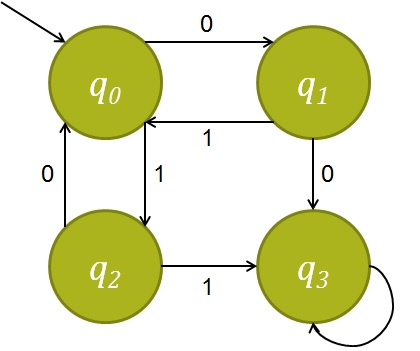
\includegraphics[width=\textwidth,height=0.8\textheight,keepaspectratio]{example}
\end{minipage}}
\begin{minipage}[c]{0.6\textwidth}
 \begin{Verbatim}[fontsize=\scriptsize]
node top(x : bool; state: int) returns (  );
var
  bias : int;
  guarantee1, guarantee2, guarantee3,
  guarantee4, guarantee5, guarantee_all : bool;
  bias_max : bool;
let
  bias = 0 -> (if x then 1 else -1) + pre(bias);
  bias_max = false ->
	(bias >= 2 or bias <= -2) or pre(bias_max);
  guarantee1 = (state = 0 => (bias = 0));
  guarantee2 = true ->
  	(pre(state = 0) and x) => state = 2;
  guarantee3 = true ->
  	(pre(state = 0) and not x) => state = 1;
  guarantee4 = bias_max => state = 3;
  guarantee5 = state = 0 or state = 1 
                    or state = 2 or state = 3;
  guarantee_all = guarantee1 and guarantee2 and
          guarantee3 and guarantee4 and guarantee5;
  --%PROPERTY guarantee_all;
  --%REALIZABLE x;
tel;
 \end{Verbatim}
\end{minipage}
\vspace{-0.5em}
\caption{Automaton and Requirements for running example}
\vspace{-2.5em}
\label{fg:example}
\end{figure}

The realizability check on this example succeeds with a k-inductive
proof of length $k = 1$. The two corresponding
$\forall\exists$-formulas ($k=0$ for the base check and $k=1$ for the
inductive check) are valid, and thus \aeval extracts two witnessing
Skolem functions that effectively describe assignments to the local
variables of the specification, as well as to \texttt{state} (see
Appendix~\ref{app:ex} for the particular formulas).

The Skolem functions are used to construct the final implementation
following the outline provided in Template~\ref{alg:synt}.
The main idea is to redefine each variable in the model
as an array of size equal to $k$ and
to use the $k$-th element of each array as the corresponding output of the call
to $k$-th Skolem function. After this initialization process, we use an infinite
loop to assign new values to the element corresponding to the last Skolem
function, to cover the inductive step of the original proof.

The final code, a snippet of which is presented below, takes 144 lines%
\footnote{Due to the space constraints, full file can be found at \url{http://www.inf.usi.ch/phd/fedyukovich/extended_example.c}}.
Since each Skolem is represented by an $\mathit{ite}$-statement (to be explained in Sect.~\ref{sec:aeval}), each its branch is further encoded into a C-code, for example:

\begin{figure}[h]
\vspace{-2em}
\begin{lstlisting}[language=C]{Name=test2}
if (((x[1] && (-1 == bias[0])) || (!x[1] && (1 == bias[0])))
     && !bias_max[0]
     && (state[0] != 0 || !x[1]) && (!state[0] != 0 || x[1])) {
  bias_max[1] = 0; bias[1] = 0; state[1] = 0;
}
\end{lstlisting}%
\vspace{-2em}
\end{figure}%


Recall that the user-defined model specifies explicitly two transitions (via \texttt{guarantee2} and \texttt{guarantee3}) only, while the set of implicitly defined transitions (via \texttt{guarantee1} and \texttt{guarantee4}) is incomplete.
%For example, the model does not specify an incoming transition to (\texttt{state = 0}).
Interestingly, our synthesized implementation turns all implicit transitions into explicit ones which makes them able to execute, and furthermore adds the missing ones (e.g., as in the aforementioned snippet, from \texttt{state = 1} to \texttt{state = 0}).

%%% Local Variables:
%%% mode: latex
%%% TeX-master: "document"
%%% End:
